\input{../../../stock/en-tete_v6.tex}

\newcommand{\titrechapitre}{Développement et factorisation}
\newcommand{\numerochapitre}{1}

\renewcommand{\headrulewidth}{0.4pt}
\renewcommand{\footrulewidth}{0.4pt}
\fancyfoot[L]{Raphaël JONTEF}
\fancyfoot[C]{\thepage}
\fancyfoot[R]{\href{https://www.alveusclub.com/}{Alveus}}
\fancyhead[L]{Mathématiques : Seconde}
\fancyhead[R]{\titrechapitre}

\begin{document}
\input{../../../stock/commands.tex}

% Page de titre custom
\begin{center}
\small Exercices issus du site \href{https://jaicompris.com/lycee/math/fonction/fonction-college.php}{jaicompris.com}\par
\end{center}

\begin{multicols}{2}
\begin{exercice}{}{}
    Traduire chaque phrase par une égalité~:
    \begin{enumeratebf}
        \item 8 a pour image 5 par la fonction $f$
        \item -2 est l'image de -5 par la fonction $f$
        \item 7 est un antécédent de 4 par la fonction $f$
    \end{enumeratebf}
\end{exercice}

\begin{exercice}{}{}
    Traduire par une phrase contenant le mot « image », puis contenant le mot « antécédent »:
    \begin{enumeratebf}
        \item $f(3)=10$
        \item $g(-4)=0$
        \item $f(5)=7$
    \end{enumeratebf}
\end{exercice}

\begin{exercice}{}{}
Modélisez chaque situation à l'aide d'une fonction:
\begin{enumeratebf}
    \item Le coût d'un trajet en taxi est de 0{,}75~€ par kilomètre, plus la prise en charge de 4~€.
    \item Le périmètre d'un rectangle de dimensions 4~cm et $x$~cm.
    \item L'aire d'un carré de côté $x$~cm.
\end{enumeratebf}
\end{exercice}

\newcolumn
\begin{exercice}{}{}
    $f$ est la fonction définie par $f(x)=3x-1$.
    \begin{enumeratebf}
        \item Calculer $f(6)$.
        \item Calculer l'image de $2$.
        \item Déterminer l'antécédent de $5$.
    \end{enumeratebf}
\end{exercice}

\begin{exercice}{}{}
    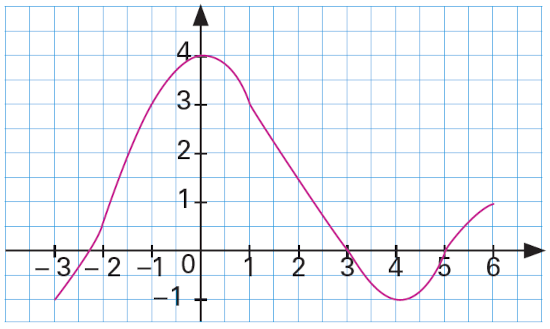
\includegraphics[width=\linewidth]{../../src/aforfjazqrfazk,crfe.png}

    Lire:
    \begin{enumeratebf}
        \item L'image de 2 par $f$.
        \item L'image de 6 par $f$.
        \item $f(5)$.
        \item Les antécédents de 3 par $f$.
    \end{enumeratebf}
\end{exercice}

\begin{exercice}{}{}
    Voici des informations sur une fonction $h$:
    \begin{align*}
        \begin{array}{ll}
        h(-3) = 3 &\quad h(0) = -2 \\
        h(-1) = 2 &\quad h(1) = -2 \\
        h(3) = 2 &\quad h(5) = 0
        \end{array}
    \end{align*}
    Quelle est l'image par la fonction $h$ des nombres $-3$, $0$ et $5$~?:
    Citer un antécédent par la fonction $h$ des nombres $-2$ et $3$~:
    Citer un nombre dont l'image par $h$ est $2$.
\end{exercice}


\end{multicols}

\begin{exercice}{}{}

\begin{enumeratebf}
    \item Recopier et compléter le tableau suivant~:\\\\
        \begin{tabular}{|l|l|}
        \hline
        Notation mathématique & En français \\
        \hline
        $f(7)=2$ & L'image de \dotuline{\hspace{1cm}} est \dotuline{\hspace{1cm}} \\
        $f(8)=-3$ & Un antécédent de \dotuline{\hspace{1cm}} est \dotuline{\hspace{1cm}} \\
        $f(\ldots)=\ldots$ & 4 a pour image 5 \\
        $f(\ldots)=\ldots$ & 1 a pour antécédent $-6$ \\
        \hline
        \end{tabular}
    \item Traduire en français l'égalité $f(-3)=4$ de deux façons différentes.
\end{enumeratebf}
    

\end{exercice}

\begin{exercice}{}{}
    Le graphique ci-dessous donne l’évolution de la température (en °C) à la station météo de Paris-Montsouris le 1er août 2020. On note $T$ la fonction qui, à l’heure, associe la température en ce lieu.
    \begin{center}
    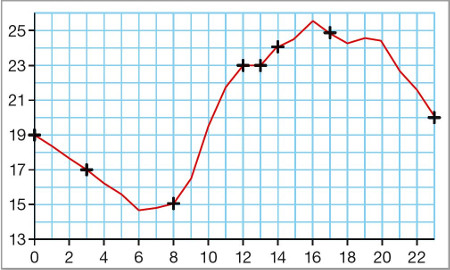
\includegraphics[width=\linewidth]{../../src/aezfaezjgfbqezojigfhf.png}
    
    \end{center}

    \begin{enumeratebf}
        \item Quelle légende peut-on écrire sur chaque axe ?
        \item Lire et interpréter : $T(8)$, $T(12)$, $T(14)$.
        \item Lire approximativement et interpréter les antécédents de 16 par la fonction $T$.
    \end{enumeratebf}
\end{exercice}

\end{document}